% LLNCStmpl.tex
% Template file to use for LLNCS papers prepared in LaTeX
%websites for more information: http://www.springer.com
%http://www.springer.com/lncs

\documentclass{llncs}
%Use this line instead if you want to use running heads (i.e. headers on each page):
%\documentclass[runningheads]{llncs}

\usepackage{amsmath}
\usepackage[BoldFont,SlantFont,CJKchecksingle]{xeCJK}
\setCJKmainfont[BoldFont=SimHei]{SimSun}
\setCJKmonofont{SimSun}% 设置缺省中文字体
\parindent 2em   %段首缩进

\begin{document}
\title{Statistics}

%If you're using runningheads you can add an abreviated title for the running head on odd pages using the following
%\titlerunning{abreviated title goes here}
%and an alternative title for the table of contents:
%\toctitle{table of contents title}

\subtitle{网易公开课-可汗学院}

%For a single author
\author{Zheng Rui}

%For multiple authors:
%\author{First Name\inst{1} \and Second Author Name\inst{2}}


%If using runnningheads you can abbreviate the author name on even pages:
%\authorrunning{abbreviated author name}
%and you can change the author name in the table of contents
%\tocauthor{enhanced author name}

%For a single institute
\institute{CSE@HKUST\\ \email{rzhengphy@gmail.com}}


% If authors are from different institutes 
%\institute{First Institute Name \email{email address} \and Second Institute Name\thanks{Thank you to...} \email{email address}}

%to remove your email just remove '\email{email address}'
% you can also remove the thanks footnote by removing '\thanks{Thank you to...}'

\maketitle

\section{Concept}
Mean=Arithmetic average, median, mode(众数, the element which appears the most), sample, population, $\mu=\sum_{i=1}^{N}x_i/N$ is population mean, $\overline{x}=\sum_{i=1}^{n}x_i/n$ is sample mean, population varience $\sigma^2=\sum_{i=1}^{N}(x_i-\mu)^2/N$, $\sigma$ is called standard deviation, sample varience $S_n^2=\sum_{i=1}^{n}(x_i-\overline{x})^2/n$, when the sample mean is close to the population mean, and the sample range and distribution is like the population range and distribution, then the sample varience is a good approximation of population varience, but when the sample mean is far from the population mean(which is not uncommon), then the sample varience will largely underestimate the population varience. The unbiased sample varience $S^2=S_{n-1}^2=\sum_{i=1}^{n}(x_i-\overline{x})^2/(n-1)$ turns out to be a much better estimator of the population varience, however, it turns out $S$ is not a good estimator of standard deviation $\sigma$.

Binomial distribution: repeat independent Bernoulli trial (e.g tossing a coin) for $n$ times, suppose some expected result (e.g head) in each Bernoulli event appears with fixed probability $p$, then the probability of the expected results appearing $k$ times is $f(k;n,p)=\binom{n}{k}p^k(1-p)^{n-k}$, when we say $X$ obeys Binomial distribution $B(n,p)$ or $b(n,p)$, actually refers to $X$ obeys pdf $f(X;n,p)$, when $p$ is not $1/2$, this disperse pdf is unsymmetric, some properties: $f(k;n,p)=f(n-k;n,1-p)$, $E[X]=np$, $Var[X]=\overrightarrow{\sigma^2}=np(1-p)$, and central limit theorem: if $n\rightarrow\infty$, then the quantity $\frac{X-np}{\sqrt{np(1-p)}}\rightarrow N(0,1)$.

Poisson distribution: $X$: number of cars passing in an hour, the probability of a car passing in each infinitimal time slice should be identical and independent. Connection with binomial distribution: suppose for poisson distribution, the expectation of the number of cars passing in an hour is $E[X]=\lambda$, suppose in each minute the probability of there is a car passing Bernoulli event is $p=\lambda/60$, equivalently we can say the average cars passing in a minute is $p=\lambda/60$, and this event trials $n=60$ times in an hour, then we have $E[X]=\lambda=n*p$, $\lambda^{cars/hour}=60^{mins/hour}*\frac{\lambda}{60}^{cars/min}$, the probability of having $k$ cars passing in an hour will be $p(X=k)=\binom{60}{k}(\frac{\lambda}{60})^k(1-\frac{\lambda}{60})^{60-k}$, what we need to do to get the poisson distribution is to devide the hour window into infinite granularity, which means $60\rightarrow\infty$, $p(X=k)=\lim_{n\rightarrow\infty}\binom{n}{k}(\frac{\lambda}{n})^k(1-\frac{\lambda}{n})^{n-k}=\lim_{n\rightarrow\infty}\frac{n(n-1)(n-2)\cdots(n-k+1)}{n^k}\frac{\lambda^k}{k!}(1-\frac{\lambda}{n})^n(1-\frac{\lambda}{n})^{-k}=\frac{\lambda^k}{k!e^\lambda}$.

Gaussian or Normal distribution: $p(x)=\frac{1}{\sqrt{2\pi}\sigma}e^{-\frac{1}{2}(\frac{x-\mu}{\sigma})^2}$, where $\frac{x-\mu}{\sigma}$ is called standard $z$ score, it means how many standard deviations that $x$ is away from $\mu$. cumulative density function(CDF) is $F(X\leq x)$. right skewed distribution = positively skewed distribution, left skewed distribution = negtively skewed distribution.
\begin{figure}
\centering
\def\svgwidth{\columnwidth}
\input{skewed.pdf_tex}
\end{figure}

``Empirical rule" also called ``$68-95-99.7$" rule, which means:
\begin{figure}
\centering
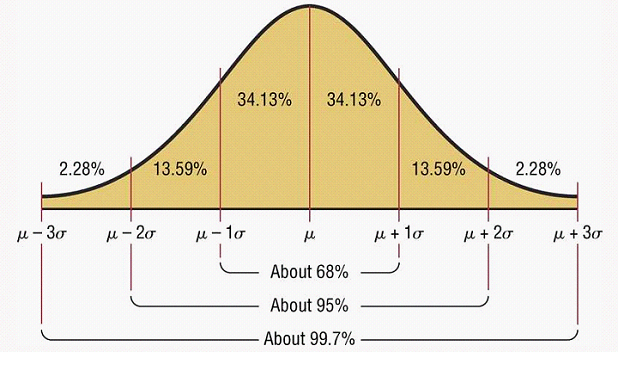
\includegraphics[width=0.8\textwidth]{EmpiricalRule.png}
\end{figure}

Standard normal distribution is $\mathcal{N}(0,1)$. 
Central limit theorem: one sample: $[X_1,X_2,\cdots,X_n]$, each random variable $X_i$ independently obeys the same $p(X)$ which has $E[X]=\mu, Var[X]=\sigma^2$, each sample has a sample mean $\overline{x_n}=\sum_{i=1}^{n}x_i/n$, if we repeat sampling for infinite times we could get a probability distribution $p(\overline{x_n})$ about $\overline{x_n}$, when $n$ is large, $p(\overline{x_n})\sim\mathcal{N}(\mu,\sigma/\sqrt{n})$, or equivalently speaking, $p(\frac{\overline{x_n}-\mu}{\sigma/\sqrt{n}})\sim\mathcal{N}(0,1)$, the $\sigma_n=\sigma/\sqrt{n}$ is called the standard error of the mean, when $n\rightarrow\infty$, which means for infinite sample size, $\lim_{n\rightarrow\infty}p(\overline{x_n})\sim\mathcal{N}(\mu,0)$. 

Kurtosis: larger kurtosis means it's more peaky, a perfect normal distribution has zero skew and zero kurtosis.
\begin{figure}
\centering
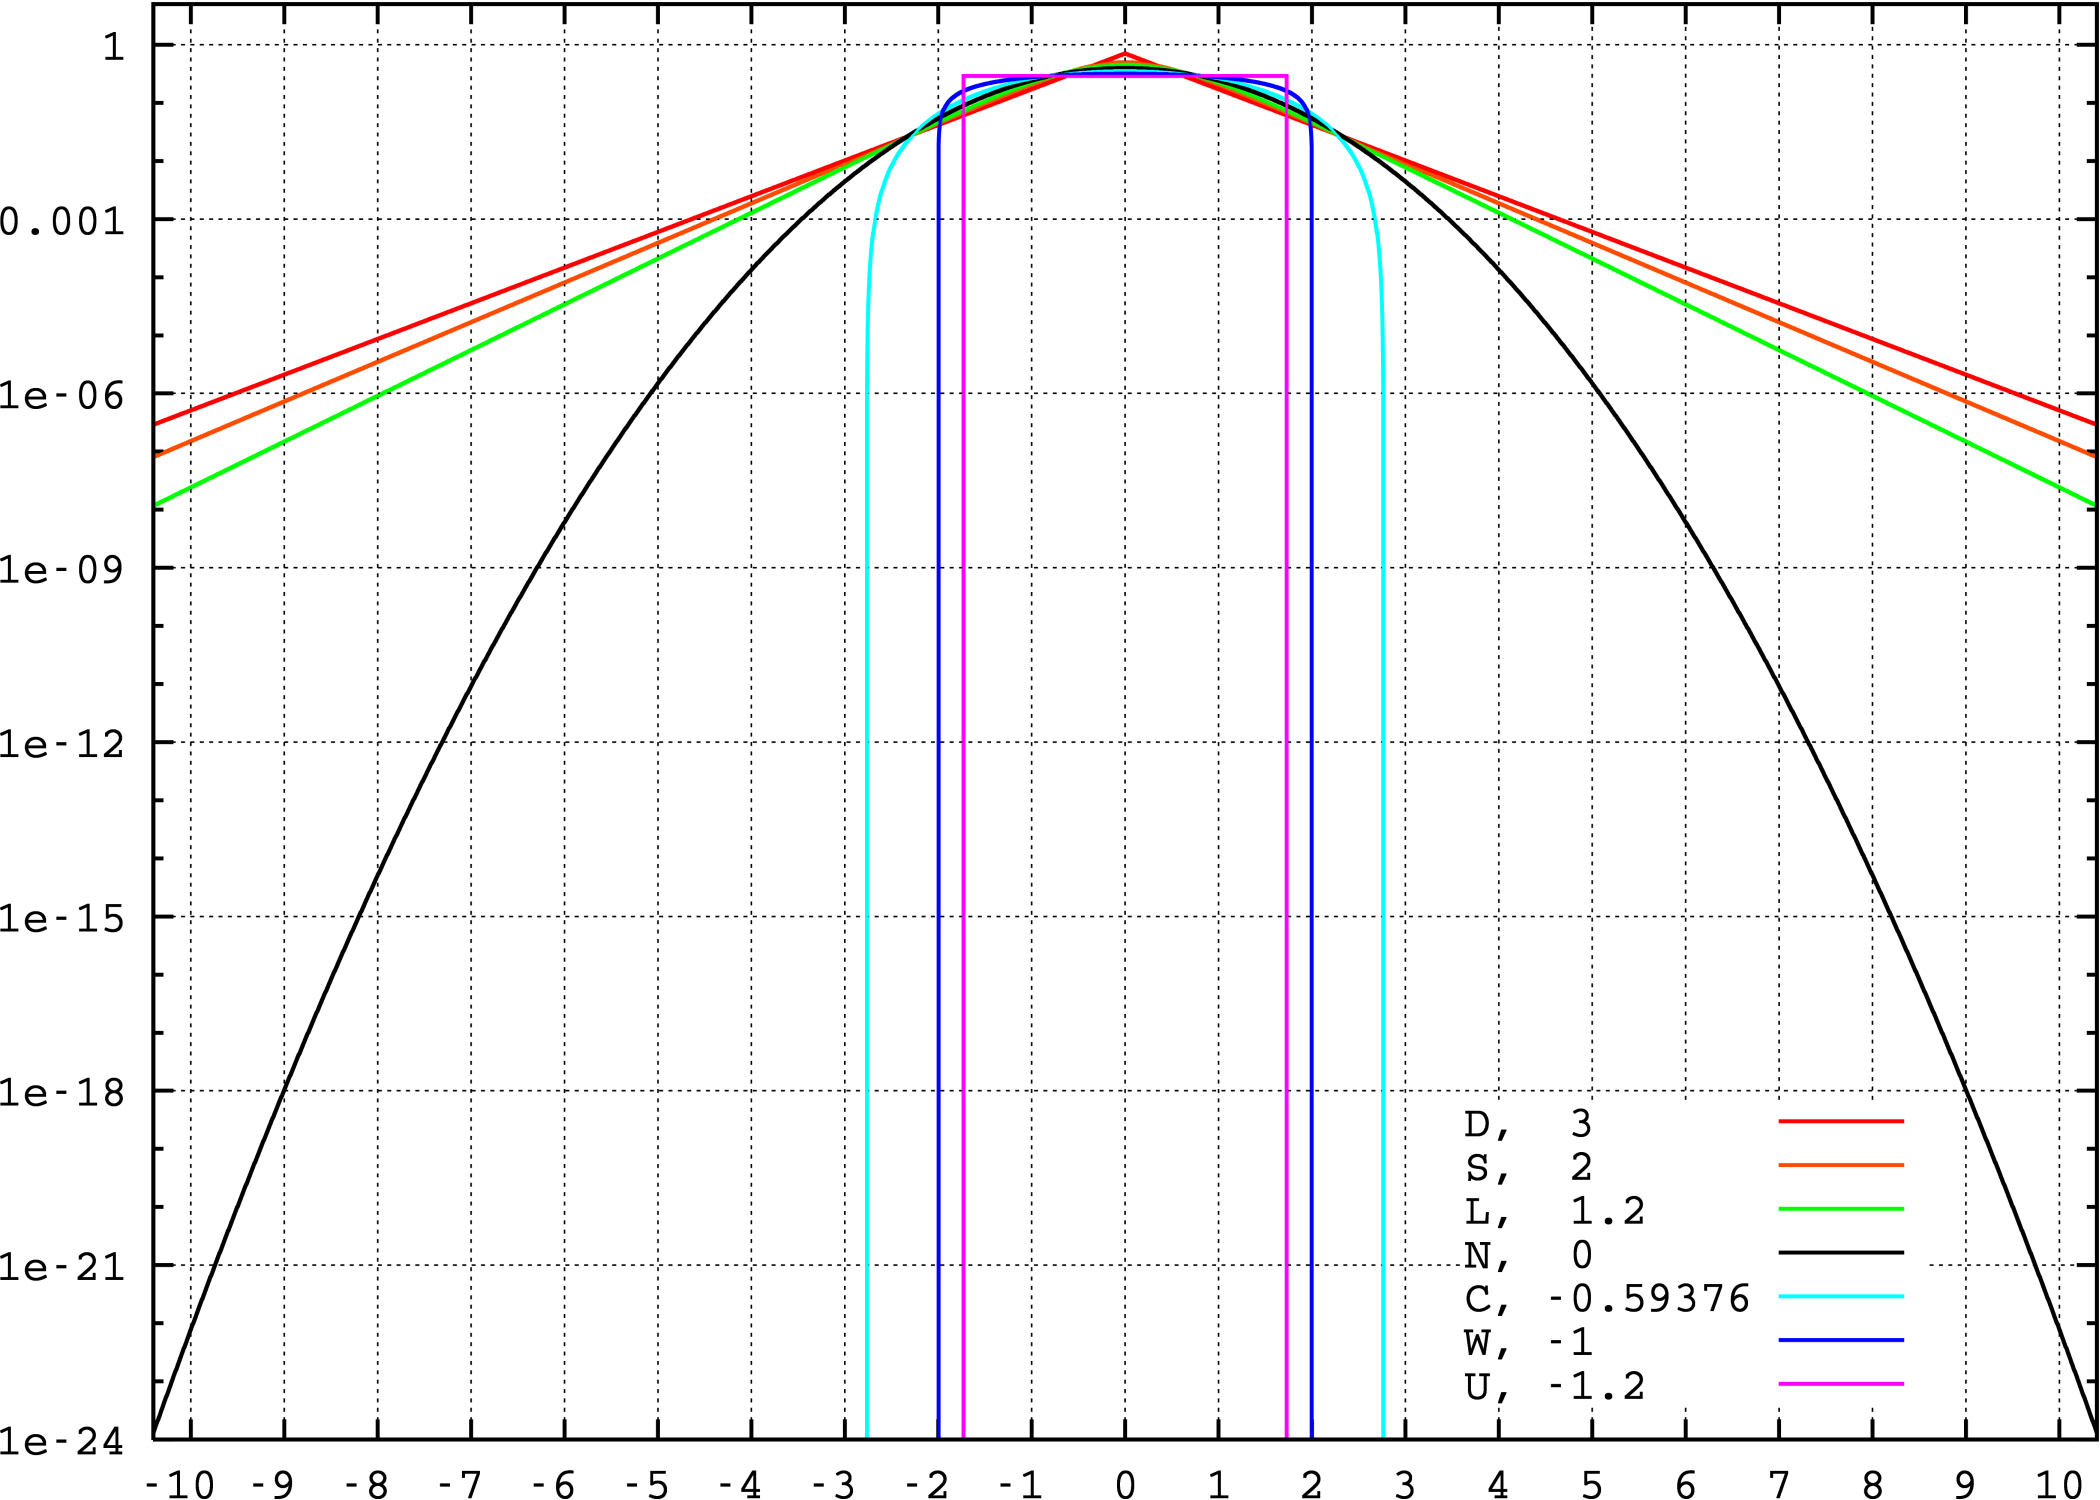
\includegraphics[width=0.6\textwidth]{kurtosis.png}
\end{figure}

Confidential interval, find an interval such that "reasonably confident" that there is a $95\%$ chance that the true $\mu$ is in that interval. suppose we have a sample of size $n$, based on this sample, we could calculate $\mu_{\overline{x}}$ and $\sigma_{\overline{x}}$, when $n>=30$, $\mu_{\overline{x}}$ and $\sigma_{\overline{x}}$ is a good approximation of population average $\mu$ and standard deviation $\sigma$, then the true result should obeys $\mathcal{N}(\mu_{\overline{x}},\sigma_{\overline{x}}/\sqrt{n})$, so the $95\%$ confidential interval $[\mu_{\overline{x}}-\delta,\mu_{\overline{x}}+\delta]$ means cumulative density in this range is $95\%$, $\delta$ is called the margin of error.

\begin{figure}
\centering
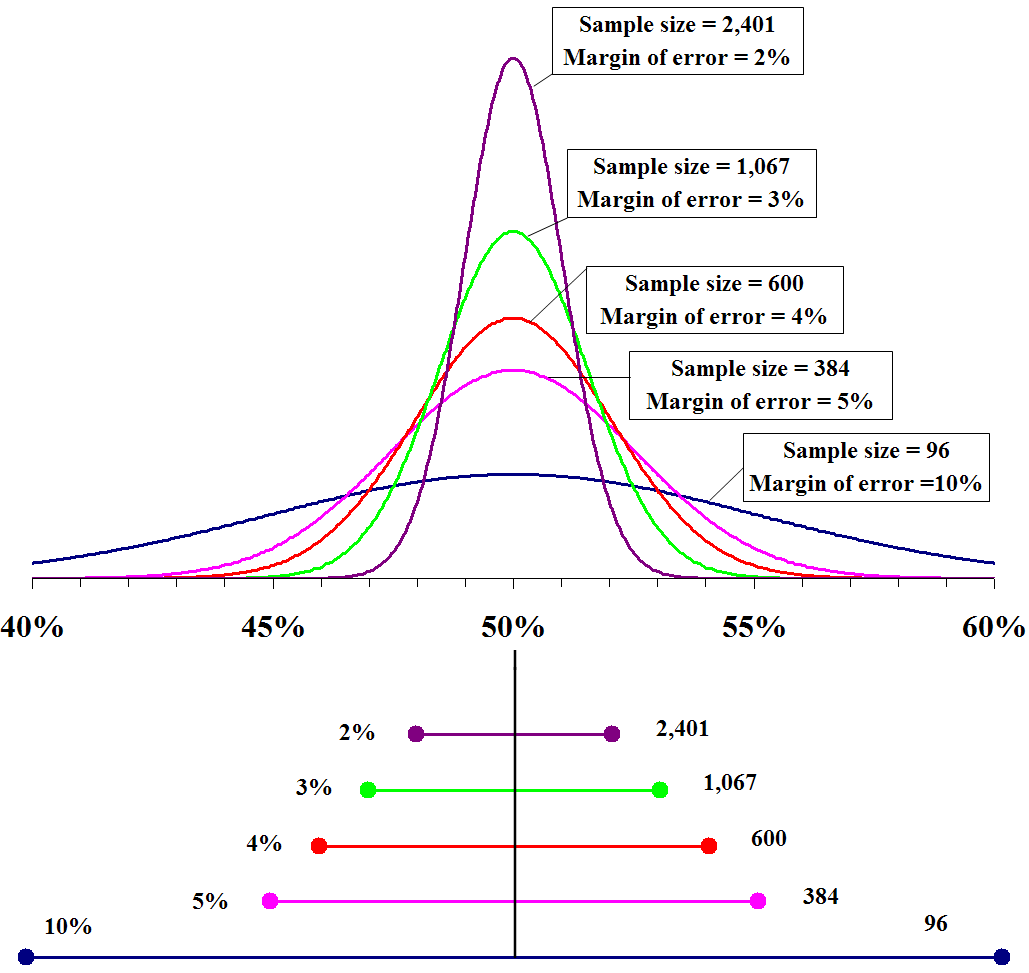
\includegraphics[width=0.6\textwidth]{Marginoferror.png}
\caption{$95\%$ confidence intervals for different sample size}
\end{figure}

When sample size $n<30$, then the sample standard deviation $S$(the $\sigma_{\overline{x}}$ above) will be a bad estimation of population standard deviation $\sigma$, and instead of using $\mathcal{N}$ distribution, we should use $\mathcal{T}$ distribution(fatter tailed in both sides than $\mathcal{N}$ distribution), but still we will use sample standard deviation $S$ in later, and isteading of looking for $Z$ table to find out the confidence intervals, we should use $T$ table to find out the confidence intervals.

\section{Details}































\iffalse
\begin{abstract}
abstract text goes here - Lorem ipsum dolor sit amet, consectetur adipiscing elit, sed do eiusmod tempor incididunt ut labore et dolore magna aliqua.
\end{abstract}

\section{First Section}

\subsection{First Subsection}
\subsubsection{First Subsubsection}
Lorem ipsum dolor sit amet, consectetur adipiscing elit, sed do eiusmod tempor incididunt ut labore et dolore magna aliqua. Ut enim ad minim veniam, quis nostrud exercitation ullamco laboris nisi ut aliquip ex ea commodo consequat. 

\subsubsection{Second Subsubsection}
Lorem ipsum dolor sit amet, consectetur adipiscing elit, sed do eiusmod tempor incididunt ut labore et dolore magna aliqua.

%Example of a numbered list
\begin{enumerate}
\item First item in list
\begin{enumerate}
\item First sub item
\item Second sub item
\end{enumerate}
\item Second item in list
\end{enumerate}

\subsection{Second Subsection}
Lorem ipsum dolor sit amet, consectetur adipiscing elit, sed do eiusmod tempor incididunt ut labore et dolore magna aliqua. Ut enim ad minim veniam, quis nostrud\cite{reference1} exercitation ullamco laboris nisi ut aliquip ex ea commodo consequat. Duis aute irure dolor in reprehenderit in voluptate velit esse cillum dolore eu fugiat nulla pariatur. Excepteur sint occaecat cupidatat non proident, sunt in culpa qui officia deserunt mollit anim id est laborum.\\
\ldots\\ 
``sdf 'fdsf' asfa''\\
www.ust.hk/$\sim$saf\\
www.ust.hk/~saf\\
www.ust.hk/\~saf\\
www.ust.hk/\~{}asf\\

\begin{displaymath}
\sum_{\substack{0<i<n \\ 1<j<m}}
P(i,j) =
\sum_{\begin{subarray}{l}
i\in I\\
1<j<m
\end{subarray}} Q(i,j)
\end{displaymath}

\begin{proposition}
Insert proposition here
\end{proposition}

\begin{proof}
Insert proof here
\end{proof}

%The bibliography, done here without a bib file
%This is the old BibTeX style for use with llncs.cls
\bibliographystyle{splncs}

%Alternative bibliography styles:
%the following does the same as above except with alphabetic sorting
%\bibliographystyle{splncs_srt}
%the following is the current LNCS BibTex with alphabetic sorting
%\bibliographystyle{splncs03}
%If you want to use a different BibTex style include [oribibl] in the document class line

\begin{thebibliography}{1}
%add each reference in here like this:
\bibitem[RE1]{reference1}
Author:
Article/Book:
Other info: (date) page numbers.
\end{thebibliography}
\fi


\end{document}

